\documentclass[12pt]{article}

%opening
\title{ChangeEngine Game Engine}
\author{By Cedric Wienold,\\
California Polytechnic Unversity,\\
San Luis Obispo, CA\\\\
Advised by Dr. Michael Haungs\\\\}
\date{\today}

\usepackage{enumerate}
\usepackage{amsmath}
\usepackage{listings}
\usepackage{graphicx}

\begin{document}
  
  \maketitle

  \thispagestyle{empty}

  \vfill

  \begin{flushright}
    
    Date Submitted:\makebox[1.5in]{\hrulefill}

    \vspace{12pt}
    
    Advisor:\makebox[1.5in]{\hrulefill}
  \end{flushright}

  \newpage
  
  \pagenumbering{roman}

  \tableofcontents

  \newpage

  \addcontentsline{toc}{section}{Abstract}
  \begin{abstract}
    We propose to design a game engine which will provide the framework for fast, simple deployment of games. We analyzed several different game engine designs to allow programmers to work on game design rather than programming the structure of windows, graphics, sounds, et cetera, but allow them to program a wide range of 2D games. The programmer will handle the logic of each interaction on his own, but trivial functions such as drawing, collision detection, and input will be handled by this engine. The engine is available as a static library programmed in C++, which gives the user the power to program in any language that can implement such a library. A major feature of this engine is pluggable functions which can be implemented by the user, such as artificial intelligence.
  \end{abstract}
  
  \newpage
  
  \pagenumbering{arabic}

  \section{Introduction}
    Game engines can be difficult to learn for a programmer who has just downloaded the libraries or source code for it. The main issues we see are that the programmer is expected to do a lot of work to get started: rudimentary operations like window creation and input detection can be hard to wrap one's mind around. Our goal is to look from a novice's point of view, with an engine which will hand-hold them through these operations until they feel able to extend my own engine's classes. We have no delusions of grandeur: If a programmer sufficiently experienced in game programming sees a need that we do not fulfill, he is free to overload it with his own code.

    We also feel that the basic logic of the program is the responsibility of whoever is programming the game. Our engine provides functions which are necessary to most games, namely collision detection, but the implementer of the engine is responsible for what happens between the objects our engine provides.

  \section{Game Engine}
    The game engine supports two main ways of implementing its classes: managed and unmanaged.
\subsection{Managed Engine}
The managed engine provides memory management benefits and ease of use at the cost of flexibility to the user. Everything the programmer creates or instantiates will be done through the overarching game engine class.

\subsubsection{Usage}
\begin{enumerate}
 \item \begin{verbatim} ChangeEngine* engine = ChangeEngine::Initiate(); \end{verbatim}
This is the overarching game engine class, through which most of our operations will take place.
 \item \begin{verbatim} engine->setWindowCaption("Test Window"); \end{verbatim}
The programmer may wish to use a custom window title, as this is a windowed application. Full screen is not yet supported.
 \item \begin{verbatim} engine->createWindow(screen_width,screen_height,bpp); \end{verbatim}
This sets up the game window with the given width, height, and color depth.
 \item \begin{verbatim} engine->createLevel("Level1"); \end{verbatim}
Scenes in this engine are split into ``Levels'', each of which contains several GameObject classes.
 \item \begin{verbatim} engine->createGameObject("Level1","Object1"); \end{verbatim}
This creates ``Object1'' and places it into ``Level1'' to be handled there.
 \item \begin{verbatim} engine->attachImageToGameObject("Level1","Object1",
"filename.png",tilewidth,tileheight); \end{verbatim}
This will attach an image to ``Object1'', also known as an 'avatar'. This is not a default operation for GameObjects, as it is likely the user will want to have an object with no image (for logical operations and such). ``tilewidth'' and ``tileheight'' are terms used in the context of tile sets, where multiple sprites of animation are contained in the same file. Sprite width and height are considered to be the same for all sprites in a tile set.
 \item \begin{verbatim} engine->addAvatarState("Level1","Object1",spritecount); \end{verbatim}
This creates a state for the avatar and sets the number of sprites in that state. In the actual image file, each state is on a single row of tiles, and the sprite count is the number of sprites available on that row of animation. In this way, the tile set can have a variable number of frames of animation for each state.

A state can be something as simple as the direction the object is facing, or an action it is taking, or both. The programmer must make sure to keep track of the order states are given, as they added from the top of the file down, and are indexed by integer starting from zero.
 \item \begin{verbatim} engine->drawObject("Level1","Object1",state,frame); \end{verbatim}
This will draw ``Object1'' of ``Level1'' to the window with the given state and frame, as given above. Going outside the bounds of the number of states added, or the number of frames in that state, will result in undefined operation.
 \item ... Game Operations ...
 \item \begin{verbatim} ChangeEngine::Destroy(); \end{verbatim}
This will make use of the game engine's internal memory management framework to remove all objects created so that the programmer need not worry about it.
\end{enumerate}

\subsection{Unmanaged Engine}
The game engine provides the programmer with unrestricted access to each class contained therein. While the programmer must do his own memory management to prevent leaks, he is not restricted to our ``Level'' framework or even our own drawing functions. What follows is only an example of what can be done with the freedom of an unmanaged engine.

\begin{enumerate}
 \item \begin{verbatim} ChangeEngine* engine = ChangeEngine::Initiate(); \end{verbatim}
 \item \begin{verbatim} engine->setWindowCaption("Test Window"); \end{verbatim}
 \item \begin{verbatim} engine->createWindow(screen_width,screen_height,bpp); \end{verbatim}
 \item \begin{verbatim} GameObject* object = new GameObject(); \end{verbatim}
 \item \begin{verbatim} object->setWidth(tilewidth); \end{verbatim}
 \item \begin{verbatim} object->setHeight(tileheight); \end{verbatim}
 \item ... Game Operations ...
 \item \begin{verbatim} object->drawImage(engine->getWindow(),state,frame); \end{verbatim}
 \item \begin{verbatim} SDL_Flip(engine->getWindow()->getScreen()); \end{verbatim}
 \item ... Game Loop until Finished ...
 \item \begin{verbatim} GameObject::Destroy(object); \end{verbatim}
 \item \begin{verbatim} engine->Destroy(); \end{verbatim}
\end{enumerate}

We have made every attempt to expose useful variables in each object. One need only browse the available header files to understand each function. For example, ChangeEngine's GameWindow class contains an SDL\_Surface called ``screen'', which we make available for use in SDL operations with \begin{verbatim}getScreen()\end{verbatim}.

Take note that the GameObject class also has its own static destruction function. In an unmanaged engine, it will be the programmer's responsibility to locate all applicable class destruction functions and use them.

\subsection{Object Controllers}
This engine uses the concept of ``controllers'' to handle objects that need to be moved for whatever reason. Every object has a private GameController instance, which is null at first, since many objects may not require being controlled. The controller depends on using a managed engine, or an effective use of GameLevels. The game engine provides \begin{verbatim}actObjects(GameLevel*)\end{verbatim} as an easy way to force all objects to be controlled, and this can be done every loop of the game engine.

The GameController class is an abstract class. In order for the programmer to control an object, he must make a new class which inherits GameController and write the \begin{verbatim}act(GameLevel*,GameObject*,EventListener*)\end{verbatim} function himself. The act() function will take in three variables: the level the object is on, the object the controller acts on, and an event listener. Not following these standards for the variables will result in wholly undefined behavior.

\subsubsection{Artificial Intelligence}
The implementation of this function can be as simple as moving the object back an forth on its own, but its access to the level makes it aware of all objects in the field, so that the programmer is able to use artificial intelligence to make the object decide its actions based on its environment.

\subsubsection{User Interaction}
The controller object also allows the programmer to have the user interact directly with the object. The reason the EventListener is included in the function is to make the object aware of events such as keypresses or mouse clicks and act accordingly.

\subsection{Sequence Diagrams}
The following diagrams show the general sequence of events using the managed engine to run a game.

\subsubsection{Initialization}
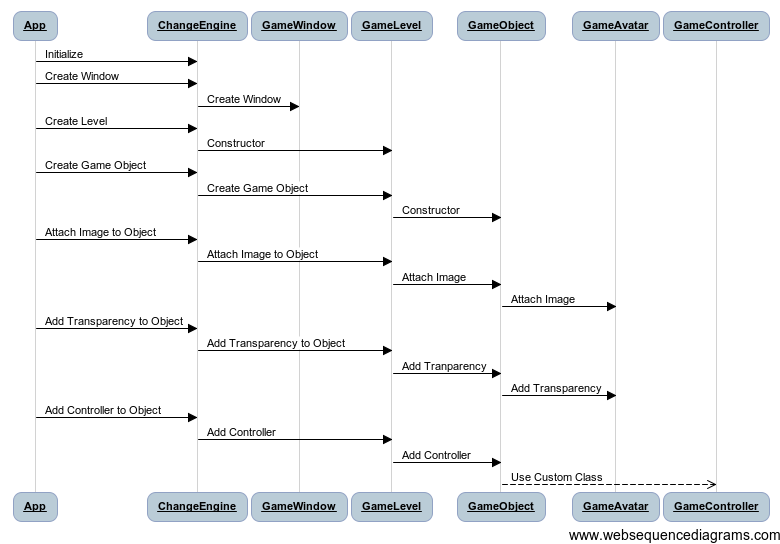
\includegraphics[width=5.9in]{init.png}

\subsubsection{Game Loop}
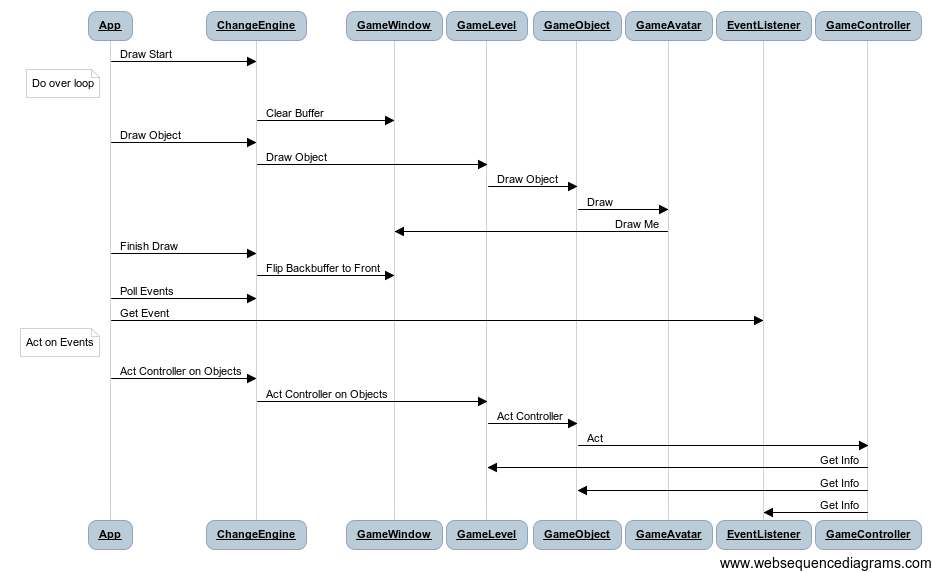
\includegraphics[width=5.9in]{loop.png}

\subsubsection{Destruction of Engine}
\includegraphics[width=4in]{destroy.png}

  \section{Design and Implementation}
    ChangeEngine will fulfill the following software requirements:

\begin{enumerate}
  \item General Requirements

  \begin{enumerate}
    \item Single library implementing all functions for a rudimentary game

    \begin{enumerate}
      \item Engine Class
      \item Window Container
      \item Level Container
      \item Game Object Container
      \item Game Avatar (Tilemap Container)
      \item Event Listener
      \item Object Controller
    \end{enumerate}

    \item Extensible classes for programmers to ``plug in'' their own logic

    \begin{enumerate}
      \item Object Controller (Artificial Intelligence or User Input)
      \item Event Handler
    \end{enumerate}

  \end{enumerate}

\end{enumerate}

  \section{Tools and Teamwork}
    This project will primarily be programmed by Cedric Wienold using various programming environments supporting C++ code. Teamwork will be limited to interviews with industry professionals concerning algorithms and class organization advice.

  \section{Analysis}
    Testing this engine is an important way of determining if its current programming is at all useful for programmers.

    To test the engine's managed object framework, I would run through a loop of progressively more objects (tens, hundreds, thousands, tens of thousands, etc.) and log the amount of time the game engine takes to create the objects, use the objects functions (such as attaching images and using the controllers on every loop), and destroy the objects.

  \section{Related Work}

  \section{Conclusions}
    The programmer must be careful to ensure his usage of this class's available functions is logical.
\subsection{ChangeEngine}
\begin{verbatim*}pollEvents()\end{verbatim*} should only be called once per loop to ensure that multiple functions depending on the same event are not deprived of it because they did not act on the event quickly enough.
\\

\begin{verbatim}createWindow(int w, int h, int bpp)\end{verbatim} should only be used with sensible, non-negative values.
\\

\begin{verbatim}createLevel()\end{verbatim} and \begin{verbatim}createGameObject\end{verbatim} have protections against being called with same-named values repeatedly. Keep in mind that if debug mode is off, the programmer will not be informed of a failure unless he is specifically checking for it.
\\

\begin{verbatim}addAvatarState()\end{verbatim} should be used on a row-by-row basis for tile sets.
\\

\begin{verbatim}drawObject()\end{verbatim} will not actually output an object to the screen.
\\

\begin{verbatim}drawFinish()\end{verbatim} is necessary to flip the backbuffer to the front, and should only be called once every loop to prevent flickering.

  \section{Future Improvements}
    This project will remain open source for any programmer to extend and improve upon it. ChangeEngine will maintain a pluggable interface in many ways so that programmers need only design their own functions and pass them into the engine if they wish to use them. Artificial intelligence, collision detection, and input detection are all areas which programmers can design their own plug-ins for.

As far as future improvements to the game engine go, the following is a noncomprehensive list:

\begin{enumerate}
 \item Change object references from strings to integers, to make loop-based instantiation easier.
 \item Use several debug modes to change terminal output.
 \item Continue building more specific error codes for all classes.
 \item Create single ``draw'' function for a level which will draw all managed objects.
 \item Handle timers or threads in ChangeEngine so the user need not be concerned with it.
 \item Include a pointer to a CollisionDetector class in every level, and implement said class.
 \item Fix the problem where the screen will not update its contents despite actual changes in Object coordinates.
 \item Improve documentation of functions not in ChangeEngine class, to improve support for non-managed implementations.
 \item Put level and object destructor access in ChangeEngine class.
 \item Expose individual GameLevel and GameObject instances to the user via the ChangeEngine class.
\end{enumerate}


  \newpage

  \appendix
  \section{Research}

  \subsection{Collision Detection}
    In an interview with Cal Poly Alumni Computer Science alumni Daniel Nutting, methods of collision detection employing best possible complexity in average cases were outlined, with worst possible complexity in edge cases being sacraficed. This method will be called the ``Grid Collision Detection'' method.

    \subsubsection{Grid Collision Detection}
      \emph{Theory: } Truly basic collision detection entails each object checking against all other objects for collision, and doing the same for every object. This leads to an average $O(n^2)$.

      The most apparent problem is repeated checks. One solution can be a stack method. For each object, push onto stack. Check collision with everything behind it.

      The next issue is restricting the number of objects to check on. If objects are not close to each other, there is no point in checking. This is where the grid comes in. For a set of objects, calculate the average X and Y coordinates, and split the field there into 4 quadrants. Do this more as is necessary for the number of objects.

  \section{Source Code}
\subsection{ChangeEngine}
\subsubsection{ChangeEngine.cpp}
\begin{lstlisting}[breaklines]
/**
 *  @file ChangeEngine.cpp
 *
 *  @date May 12, 2011
 *  @author Cedric Wienold
 */

#ifdef DEBUG
    #include <stdlib.h>
#endif

#include "ChangeEngine.hpp"
#include <stdio.h>

// Set singleton to null at start
ChangeEngine* ChangeEngine::pInstance = NULL;

ChangeEngine::ChangeEngine() {

   window = NULL;
}

ChangeEngine* ChangeEngine::Initiate(void) {

   #ifdef DEBUG
   fprintf(stderr,"ChangeEngine: Initiate\n");
   #endif

   //Initiate ChangeEngine if it doesn't already exist
   if (pInstance == NULL) {

      #ifdef DEBUG
         fprintf(stderr,"ChangeEngine: ChangeEngine Singleton does not exist. Creating.\n");
      #endif
      pInstance = new ChangeEngine();
   }

   //Create event listener
   if (pInstance->listener == NULL) {

      pInstance->listener = new EventListener();
   }


   #ifdef DEBUG
      fprintf(stderr,"ChangeEngine: ChangeEngine Singleton Returned\n");
   #endif

   return pInstance;
}

void ChangeEngine::Destroy(void) {

   #ifdef DEBUG
   fprintf(stderr,"ChangeEngine: Destroy\n");
   #endif

   // Clean up engine objects
   
   //If this engine is initialized
   if (pInstance != NULL) {
      
      //Destroy any levels in the array
      for(std::map<std::string,GameLevel*>::iterator it=pInstance->levels.begin(); it!=pInstance->levels.end(); it++) {
         
         #ifdef DEBUG
         fprintf(stderr,"GameEngine: Destroying level %s.\n",(*it).first.c_str());
         #endif

         GameLevel::Destroy((*it).second);
      }
      
      //See if the GameWindow has been initialized
      if (pInstance->window != NULL) {
         
         #ifdef DEBUG
         fprintf(stderr,"ChangeEngine: Window has been initialized. Destroying.\n");
         #endif
         
         GameWindow::Destroy();
      }
      #ifdef DEBUG
      else {
         
         fprintf(stderr,"ChangeEngine: Window not created yet. Not destroying.\n");
      }
      #endif

      //Destroy the game engine instance
      delete pInstance;
   }
}

int ChangeEngine::createWindow(int w, int h, int bpp) {
   
   return this->createWindow(0,0,w,h,bpp);
}

int ChangeEngine::createWindow(int x, int y, int w, int h, int bpp) {

   #ifdef DEBUG
   fprintf(stderr,"ChangeEngine: CreateWindow\n");
   #endif
   
   //Create game window
   window = GameWindow::Initiate(pInstance);

   int result = window->CreateWindow(x,y,w,h,bpp);

   if (window == NULL) {

      #ifdef DEBUG
      fprintf(stderr,"ChangeEngine: EINITIATE_FAILED\n");
      #endif
      
      return EINITIATE_FAILED;
   }

   if (result != EENGINE_SUCCESS) {

         #ifdef DEBUG
         fprintf(stderr,"ChangeEngine: EWINDOW_FAILED\n");
         #endif
   
         return EWINDOW_FAILED;
   }

   return EENGINE_SUCCESS;
}

GameWindow* ChangeEngine::getWindow() {

   return window;
}

EventListener* ChangeEngine::getEventListener() {

   return listener;
}

void ChangeEngine::setWindowCaption(const char* caption) {

   SDL_WM_SetCaption(caption,NULL);
}


int ChangeEngine::createLevel(const char* levelName) {
   
   #ifdef DEBUG
   fprintf(stderr,"GameEngine: Creating level %s.\n",levelName);
   #endif
   
   //Make sure the level name doesn't already exist
   if(levels.find(levelName) == levels.end()) {
      
      #ifdef DEBUG
      fprintf(stderr,"GameEngine: Level %s is unique, creating.\n",levelName);
      #endif
      
      levels[levelName] = new GameLevel();
   }
   #ifdef DEBUG
   else {
      
      fprintf(stderr,"GameEngine: Level %s already exists. This ain't right.",levelName);
      return ELEVELCREATE_ALREADY_EXISTS;
   }
   #endif
   
   return EENGINE_SUCCESS;
}

int ChangeEngine::createGameObject(const char* levelName, const char* objectName) {
   
   #ifdef DEBUG
   fprintf(stderr,"GameEngine: Creating Object (%s:%s)\n",levelName,objectName);
   #endif
   
   //If the level doesn't exist, this is bad
   if(levels.find(levelName) == levels.end()) {
      
      #ifdef DEBUG
      fprintf(stderr,"GameEngine: Uh oh, level %s DOESN'T EXIST\n",levelName);
      #endif
      
      return EOBJECTCREATE_INVALID_LEVEL;
   }
            
   //Make object in level
   if ((levels[levelName]->createGameObject(objectName)) != EENGINE_SUCCESS) {
      
      return EOBJECTCREATE_CREATE_FAILED;
   }
   
   return EENGINE_SUCCESS;
}

int ChangeEngine::attachImageToGameObject(std::string level, std::string object, std::string filename, int tileWidth, int tileHeight) {

   #ifdef DEBUG
   fprintf(stderr,"GameEngine: Attaching image \"%s\" to object (%s:%s)\n",filename.c_str(),level.c_str(),object.c_str());
   #endif
   
   //Check if level exists
   if (levels.find(level) == levels.end())
   {
      #ifdef DEBUG
      fprintf(stderr,"GameEngine: Uh oh, level %s DOESN'T EXIST\n",level.c_str());
      #endif
      
      return EATTACHIMAGE_INVALID_LEVEL;
   }
   
   if ((levels[level]->attachImage(object,filename,tileWidth,tileHeight)) != EENGINE_SUCCESS) {
      
      return EATTACHIMAGE_FAILED;
   }

   return EENGINE_SUCCESS;
}
int ChangeEngine::addAvatarState(std::string level, std::string object, int frameCount) {
   
   #ifdef DEBUG
   fprintf(stderr,"GameEngine: Adding state\n");
   #endif
   
   //Check if level exists
   if (levels.find(level) == levels.end())
   {
      #ifdef DEBUG
      fprintf(stderr,"GameEngine: Uh oh, level %s DOESN'T EXIST\n",level.c_str());
      #endif
      
      return EADDSTATE_INVALID_LEVEL;
   }
   
   if ((levels[level]->addAvatarState(object,frameCount)) != EENGINE_SUCCESS) {
      
      return EADDSTATE_FAILED;
   }

   return EENGINE_SUCCESS;
}

int ChangeEngine::drawObject(std::string level, std::string object, int state, int frame) {
   
   #ifdef DEBUG
   fprintf(stderr,"ChangeEngine: Drawing %s to level %s\n",object.c_str(),level.c_str());
   #endif

   if (levels.find(level) == levels.end()) {
      
      return EENGINE_FAILURE;
   }
   
   if ((levels[level]->drawObject(window,object,state,frame)) != EENGINE_SUCCESS) {
      
      return EENGINE_FAILURE;
   }
   
   return EENGINE_SUCCESS;
}

int ChangeEngine::drawStart() {
   
   SDL_FillRect(this->window->getScreen(), &(this->window->getScreen())->clip_rect, SDL_MapRGB(this->window->getScreen()->format, 0x00, 0x00, 0x00));
   
   return EENGINE_SUCCESS;
}

int ChangeEngine::drawFinish() {
   
   //Complete the drawing process
   SDL_Flip(window->getScreen());
   
   return EENGINE_SUCCESS;
}

int ChangeEngine::attachControllerToGameObject(const char* level, const char* object, GameController* controller) {

   levels[level]->attachController(object, this->listener, controller);

   return EENGINE_SUCCESS;
}

int ChangeEngine::pollEvent() {

   if (!(listener->pollEvent()))
      return EENGINE_FAILURE;

   return EENGINE_SUCCESS;
}

int ChangeEngine::actObjects(const char* level) {

   levels[level]->actObjects(this->getEventListener());
   
   return EENGINE_SUCCESS;
}

int ChangeEngine::addTransparency(const char* level, const char* object, int r, int g, int b) {
   
   if (levels[level]->addTransparency(object,r,g,b) != EENGINE_SUCCESS) {
      
      return EENGINE_FAILURE;
   }
   
   return EENGINE_SUCCESS;
}

GameLevel* ChangeEngine::getLevel(const char* level) {
   
   return levels[level];
}
\end{lstlisting}
\subsubsection{ChangeEngine.hpp}
\begin{lstlisting}[breaklines]
#include "mitlicense.hpp"

/**
 * @file ChangeEngine.hpp
 * Game engine which handles most game elements.
 *
 * @date May 12, 2011
 * @author Cedric Wienold
 */

#ifndef CHANGEENGINE_HPP_
#define CHANGEENGINE_HPP_

#include <map>
#include <string>

#include "debug.hpp"

#include "GameWindow.hpp"
#include "GameObject.hpp"
#include "GameLevel.hpp"
#include "GameController.hpp"
#include "EventListener.hpp"
#include "EventTypes.hpp"
#include "errorcodes.hpp"

/**
 * Main class of ChangeEngine which handles game elements.
 */
class ChangeEngine {
   public:

      /**
       * Construct the engine with a null window.
       */
      ChangeEngine();

      /**
       * Initiates the engine if it is not already initiated and returns a pointer to its singleton.
       * @return A pointer to the game engine object, or NULL on failure.
       */
      static ChangeEngine* Initiate();

      /**
       * Shuts down the game engine and removes it from memory.
       * This function will make every effort to detect leftover engine-created objects
       * and destroy them before exiting.
       */
      static void Destroy();


      /**
       * Create the game engine's window with the given width and heigh at (0,0).
       * @param w The window's width.
       * @param h The window's height.
       * @param bpp The window's color depth.
       * @return True if creation was successful. False otherwise.
       */
      int createWindow(int w, int h, int bpp);

      /**
       * Create the game engine's window with the given width and heigh at (x,y).
       * @param w The window's width.
       * @param h The window's height.
       * @param x The x coordinate of the window on the screen.
       * @param y The y coordinate of the window on the screen.
       * @param bpp The window's color depth.
       * @return True if creation was successful. False otherwise.
       */
      int createWindow(int x, int y, int w, int h, int bpp);

      /**
       * Return the game engine's window.
       * @return The game engine's window, or NULL if it does not exist.
       */
      GameWindow* getWindow();

      /**
       * TODO: Build functions to access listener without needing to return it here.
       */
      EventListener* getEventListener();

      /**
       * Sets the title text of the game window.
       * @param caption The desired text of the game window.
       */
      void setWindowCaption(const char* caption);
      
      /**
       * Creates a level for the game engine to manage.
       * @param levelName The custom name of the level to create. Your choice here.
       */
      int createLevel(const char* levelName);
      
      /**
       * Create a managed object for a given level.
       */
      int createGameObject(const char* levelName, const char* objectName);
      
      /**
       * Attach an image to a game object's avatar with a given filename.
       * @param level Name of level to attach image to.
       * @param object Name of object ot attach image to.
       * @param filename Filename of image to attach to object.
       * @param tileWidth Width of a single tile in the image.
       * @param tileHeight Height of a single tile in the image.
       */
      int attachImageToGameObject(std::string level, std::string object, std::string filename, int tileWidth, int tileHeight);
      
      /**
       * Add a state to the avatar tileset manager. A state will be a single row on the tileset.
       * The parameter will be the number of frames on that row. Add states from the top of the
       * tile set to the bottom, in that order specifically.
       * @param frameCount The number of frames on the current row of the tile set.
       */
      int addAvatarState(std::string level, std::string object, int frameCount);
      
      /**
       * Draw an object in a level of the given state and frame to the backbuffer. This will not
       * actually draw anything to the front buffer. To complete drawing, call draw().
       */
      int drawObject(std::string level, std::string object, int state, int frame);
      
      /**
       * Begin the drawing process.
       */
      int drawStart();
      
      /**
       * Complete the drawing process.
       */
      int drawFinish();
      
      /**
       * Attach a controller to the given game object of the given leve.
       */
      int attachControllerToGameObject(const char* level, const char* object, GameController* controller);
      
      /**
       * Poll the event buffer.
       */
      int pollEvent();
      
      /**
       * Runs controller on all objects that have one.
       */
      int actObjects(const char* level);

      /**
       * Sets the transparency color of the given object to the given RGB values.
       */
      int addTransparency(const char* level, const char* object, int r, int g, int b);
      
      GameLevel* getLevel(const char* level);
      
   private:

      /**
       * The game engine's singleton.
       */
      static ChangeEngine* pInstance;

      /**
       * Window for the game engine.
       */
      GameWindow *window;

      /**
       * Event listener
       */
      EventListener *listener;
      
      //// Now for managed objects, so the user need not care about lots of crap for memory handling
      
      /**
       * Array of levels.
       */
      std::map<std::string,GameLevel*> levels;
};

#endif /* CHANGEENGINE_H_ */
\end{lstlisting}
\subsubsection{debug.hpp}
\begin{lstlisting}[breaklines]
#define DEBUG
\end{lstlisting}
\subsubsection{errorcodes.hpp}
\begin{lstlisting}[breaklines]
#include "mitlicense.hpp"

/**
 * @file type.hpp
 * Error code declarations.
 *
 * @date May 9, 2011
 * @author Cedric Wienold
 */

#ifndef _ERRORCODES_HPP
#define _ERRORCODES_HPP

/**
 * Yeah this means "basically perfect" in all contexts.
 */
#define EENGINE_SUCCESS                0
#define EENGINE_FAILURE                99999       /* Don't use this so much. It's a placeholder for more specific errors */

/***************************
 * ChangeEngine Errors     *
 ***************************/
#define EWINDOW_FAILED                 1           /* Window creation failed */
#define EINITIATE_FAILED               2           /* Multimedia Library Initialization failed */
#define ELEVELCREATE_FAILED            3           /* Creation of a game level has failed */
#define ELEVELCREATE_ALREADY_EXISTS    4           /* Game level creation attempt on preexisting name */
#define EOBJECTCREATE_INVALID_LEVEL    5           /* Object create attempt on level that doesn't exist */
#define EATTACHIMAGE_INVALID_LEVEL     6           /* Attaching image to invalid level */
#define EATTACHIMAGE_INVALID_OBJECT    7           /* Attaching image to invalid object */
#define EOBJECTCREATE_CREATE_FAILED    8           /* Object create attempt failed */
#define EATTACHIMAGE_FAILED            9           /* Attaching of image to object failed */
#define EADDSTATE_INVALID_LEVEL        10          /* Attempted adding state to avatar of invalid level */
#define EADDSTATE_FAILED               11          /* Attempt to add state to avatar failed. */

/***************************
 * GameWindow Errors       *
 ***************************/
#define ESETVIDEOMODE_FAILED           20

/***************************
 * GameObject Errors       *
 ***************************/
#define EOBJECT_ALREADY_EXISTS         40
#define EATTACH_AVATAR_ALREADY_EXISTS  41

/***************************
 * GameLevel Errors       *
 ***************************/
#define EADDSTATE_INVALID_OBJECT       60


#endif /* _ERRORCODES_HPP */
\end{lstlisting}
\subsubsection{EventListener.cpp}
\begin{lstlisting}[breaklines]
/**
 *  @file EventListener.cpp
 *
 *  @date May 21, 2011
 *  @author Cedric Wienold
 */

#include "debug.hpp"

#include "EventListener.hpp"
#include "EventTypes.hpp"
#include "errorcodes.hpp"

bool EventListener::pollEvent() {

   return SDL_PollEvent(&event);
}

int EventListener::getEvent() {

   return event.type;
}

int EventListener::getKey() {

   return event.key.keysym.sym;
}
\end{lstlisting}
\subsubsection{EventListener.hpp}
\begin{lstlisting}[breaklines]
#include "mitlicense.hpp"

/**
 * @file EventListener.hpp
 * Listener used for grabbing events.
 *
 * @date May 21, 2011
 * @author Cedric Wienold
 */

#ifndef _EVENTLISTENER_HPP
#define _EVENTLISTENER_HPP

#include "SDL/SDL.h"

class EventListener {
   public:
      /**
       * Poll the system for events. This is generally run in a loop for as long as you wish to
       * listen for events.
       */
      bool pollEvent();

      /**
       * Receive the currently held event.
       * @return Event that the listener has heard.
       */
      int getEvent();

      /**
       * If the event is a keypress, this will return which key.
       * @return The keypress triggering the event.
       */
      int getKey();
   private:
      SDL_Event event;
};

#endif /* _EVENTLISTENER_HPP */
\end{lstlisting}
\subsubsection{EventTypes.hpp}
\begin{lstlisting}[breaklines]
#include "mitlicense.hpp"

/**
 * @file EventTypes.hpp
 * Defined types for events for use with this engine.
 *
 * @date May 21, 2011
 * @author Cedric Wienold
 */

// TODO: This is a non-comprehensive list of events. Finish it.

/** Main Events */
#define CE_QUIT         SDL_QUIT
#define CE_KEYDOWN      SDL_KEYDOWN
#define CE_KEYUP        SDL_KEYUP
#define CE_MOUSEMOTION  SDL_MOUSEMOTION
#define CE_MOUSEDOWN    SDL_MOUSEDOWN
#define CE_MOUSEUP      SDL_MOUSEUP

// TODO: Finish defining these keyboard events out of comments
/** Keyboard Events */
//Format: CE_KB_[key_identifier]
#define CE_KB_RETURN             SDLK_RETURN
#define CE_KB_ENTER              SDLK_RETURN
#define CE_KB_ESCAPE             SDLK_ESCAPE
#define CE_KB_SPACE              SDLK_SPACE
#define CE_KB_UP                 SDLK_UP
#define CE_KB_DOWN               SDLK_DOWN
#define CE_KB_RIGHT              SDLK_RIGHT
#define CE_KB_LEFT               SDLK_LEFT
/*
SDLK_BACKSPACE
SDLK_TAB
SDLK_CLEAR
SDLK_PAUSE
SDLK_EXCLAIM
SDLK_QUOTEDBL
SDLK_HASH
SDLK_DOLLAR
SDLK_AMPERSAND
SDLK_QUOTE
SDLK_LEFTPAREN
SDLK_RIGHTPAREN
SDLK_ASTERISK
SDLK_PLUS
SDLK_COMMA
SDLK_MINUS
SDLK_PERIOD
SDLK_SLASH
SDLK_0
SDLK_1
SDLK_2
SDLK_3
SDLK_4
SDLK_5
SDLK_6
SDLK_7
SDLK_8
SDLK_9
SDLK_COLON
SDLK_SEMICOLON
SDLK_LESS
SDLK_EQUALS
SDLK_GREATER
SDLK_QUESTION
SDLK_AT
SDLK_LEFTBRACKET
SDLK_BACKSLASH
SDLK_RIGHTBRACKET
SDLK_CARET
SDLK_UNDERSCORE
SDLK_BACKQUOTE
SDLK_a
SDLK_b
SDLK_c
SDLK_d
SDLK_e
SDLK_f
SDLK_g
SDLK_h
SDLK_i
SDLK_j
SDLK_k
SDLK_l
SDLK_m
SDLK_n
SDLK_o
SDLK_p
SDLK_q
SDLK_r
SDLK_s
SDLK_t
SDLK_u
SDLK_v
SDLK_w
SDLK_x
SDLK_y
SDLK_z
SDLK_DELETE
SDLK_KP0
SDLK_KP1
SDLK_KP2
SDLK_KP3
SDLK_KP4
SDLK_KP5
SDLK_KP6
SDLK_KP7
SDLK_KP8
SDLK_KP9
SDLK_KP_PERIOD
SDLK_KP_DIVIDE
SDLK_KP_MULTIPLY
SDLK_KP_MINUS
SDLK_KP_PLUS
SDLK_KP_ENTER
SDLK_KP_EQUALS
SDLK_INSERT
SDLK_HOME
SDLK_END
SDLK_PAGEUP
SDLK_PAGEDOWN
SDLK_F1
SDLK_F2
SDLK_F3
SDLK_F4
SDLK_F5
SDLK_F6
SDLK_F7
SDLK_F8
SDLK_F9
SDLK_F10
SDLK_F11
SDLK_F12
SDLK_F13
SDLK_F14
SDLK_F15
SDLK_NUMLOCK
SDLK_CAPSLOCK
SDLK_SCROLLOCK
SDLK_RSHIFT
SDLK_LSHIFT
SDLK_RCTRL
SDLK_LCTRL
SDLK_RALT
SDLK_LALT
SDLK_RMETA
SDLK_LMETA
SDLK_LSUPER
SDLK_RSUPER
SDLK_MODE
SDLK_COMPOSE
SDLK_HELP
SDLK_PRINT
SDLK_SYSREQ
SDLK_BREAK
SDLK_MENU
SDLK_POWER
SDLK_EURO
SDLK_UNDO
*/
\end{lstlisting}
\subsubsection{GameAvatar.cpp}
\begin{lstlisting}[breaklines]
/**
 * @file GameAvatar.cpp
 *
 * @date May 22, 2011
 * @author Cedric Wienold
 */

#include "GameAvatar.hpp"
#include "SDL/SDL_image.h"
#include "errorcodes.hpp"
#include "debug.hpp"

GameAvatar::~GameAvatar() {

   #ifdef DEBUG
   fprintf(stderr,"GameAvatar: Destructing avatar.\n");
   #endif

   if (tileSet != NULL) {
      
      SDL_FreeSurface(tileSet);
   }
}

SDL_Surface* GameAvatar::loadImage(const char* filename) {

   // Algorithm source: http://lazyfoo.net/SDL_tutorials/lesson03/linux/cli/index.php
   SDL_Surface* loadedImage = NULL;

   SDL_Surface* optimizedImage = NULL;

   loadedImage = IMG_Load(filename);

   if (loadedImage != NULL) {

      //Create optimized image
      optimizedImage = SDL_DisplayFormat(loadedImage);

      //Free old image
      SDL_FreeSurface(loadedImage);
   }

   return optimizedImage;
}

int GameAvatar::attachImage(std::string filename, int tileWidth, int tileHeight) {

   #ifdef DEBUG
   fprintf(stderr,"GameAvatar: Attaching image %s\n",filename.c_str());
   #endif
   
   tileSet = GameAvatar::loadImage(filename.c_str());
   
   if (tileSet == NULL) {
      
      return EATTACHIMAGE_FAILED;
   }
   
   this->tileWidth = tileWidth;
   this->tileHeight = tileHeight;
   
   return EENGINE_SUCCESS;
}

int GameAvatar::addAvatarState(int frameCount) {

   #ifdef DEBUG
   fprintf(stderr,"GameAvatar: Adding state\n");
   #endif
   
   frameSet.push_back(frameCount);
   
   return EENGINE_SUCCESS;
}

int GameAvatar::drawObject(GameWindow* window, int x, int y, int state, int frame) {
   
   SDL_Rect *srcrect = new SDL_Rect();
   SDL_Rect *dstrect = new SDL_Rect();
   
   //Position the crop rect around the frame we want
   srcrect->x = state*tileWidth;
   srcrect->y = frame*tileHeight;
   srcrect->w = tileWidth;
   srcrect->h = tileHeight;
   
   #ifdef DEBUG
   fprintf(stderr,"GameAvatar: Drawing object to (%ix%i),(%i,%i)\n",x,y,state,frame);
   #endif

   //Now we totally want to set the destination rect for the output
   dstrect->x = x;
   dstrect->y = y;
   dstrect->w = tileWidth;
   dstrect->h = tileHeight;
   
   //Blit to the window's surface
   //SDL_BlitSurface(tileSet,&srcrect,window->getScreen(),&dstrect);
   SDL_BlitSurface(tileSet,srcrect,window->getScreen(),dstrect);
   
   delete srcrect;
   delete dstrect;
   
   return EENGINE_SUCCESS;
}

int GameAvatar::addTransparency(int r, int g, int b) {
   
   if (this->tileSet == NULL)
      return EENGINE_FAILURE;
   
   int colorkey = SDL_MapRGB(this->tileSet->format, r, g, b);
   
   SDL_SetColorKey(this->tileSet, SDL_SRCCOLORKEY, colorkey);
   
   return EENGINE_SUCCESS;
}
\end{lstlisting}
\subsubsection{GameAvatar.hpp}
\begin{lstlisting}[breaklines]
#include "mitlicense.hpp"

/**
 * @file GameAvatar.hpp
 * This class describes a 2-D sprite-based avatar built with a tile set. Its only function to to
 * maintain the tile set, and draw it out on request.
 *
 * The frames are stored with one state per row. Every call for the next frame will loop through
 * the available frames in that row/state.
 *
 * When constructing the tile set, the user must add each state row separately with the number of
 * frames it holds.
 *
 * @date May 22, 2011
 * @author Cedric Wienold
 */

#ifndef GAMEAVATAR_HPP_
#define GAMEAVATAR_HPP_

#include <string>
#include <vector>
#include "SDL/SDL.h"
#include "SDL/SDL_image.h"
#include "GameWindow.hpp"

class GameAvatar {
   private:
      SDL_Surface *tileSet;
      int tileWidth,tileHeight;

      std::vector<int> frameSet;

      static SDL_Surface* loadImage(const char* filename);
      
   public:
      virtual ~GameAvatar();
      
      int attachImage(std::string filename, int tileWidth, int tileHeight);
      
      int addAvatarState(int frameCount);
      
      int drawObject(GameWindow* window, int x, int y, int state, int frame);
      
      SDL_Surface *getSurface() {return tileSet;}
      
      int addTransparency(int r, int g, int b);
};

#endif /* GAMEAVATAR_HPP_ */
\end{lstlisting}
\subsubsection{GameController.hpp}
\begin{lstlisting}[breaklines]
/**
 * @file GameController.hpp
 * Interface for classes which will control the actions of GameObjects.
 *
 * @date May 21, 2011
 * @author Cedric Wienold
 */

#ifndef _GAMECONTROLLER_HPP
#define _GAMECONTROLLER_HPP

class GameObject;
class GameLevel;

#include "GameLevel.hpp"
#include "EventListener.hpp"

class GameController {
   
   public:
   
      /**
       * Gives the object instructions on how to act given the conditions of the GameLevel.
       * 
       * @param level The current level to give the object a basis upon which to act.
       * @param object The same object that contains this controller, which will be controlled.
       */
      virtual void act(GameLevel* level, GameObject* object, EventListener* listener) = 0;
};

#endif /* _GAMECONTROLLER_HPP */
\end{lstlisting}
\subsubsection{GameLevel.cpp}
\begin{lstlisting}[breaklines]
/**
 *  @file GameLevel.cpp
 *
 *  @date May 12, 2011
 *  @author Cedric Wienold
 */

#include "GameLevel.hpp"

GameLevel::GameLevel() {
   
   width = height = 0;
}

void GameLevel::Destroy(GameLevel* level) {

   #ifdef DEBUG
   fprintf(stderr,"GameLevel: Destroying level.\n");
   #endif
   
   //Go through managed objects array and destroy each one.
   for(std::map<std::string,GameObject*>::iterator it = level->objects.begin(); it != level->objects.end(); it++) {
      
      //Sanity check
      if ((*it).second != NULL) {
	 
	 #ifdef DEBUG
	 fprintf(stderr,"GameLevel: Destroying object %s.\n",(*it).first.c_str());
	 #endif
   
	 //This is where I would call GameObject::Destroy(*it) or something along those lines
	 GameObject::Destroy((*it).second);
      }
   }
   
   delete level;
}

int GameLevel::createGameObject(std::string objectName) {

   //make sure object doesn't already exist here
   if (objects.find(objectName.c_str()) != objects.end()) {
      
      #ifdef DEBUG
      fprintf(stderr,"GameLevel: Object %s already exists.\n",objectName.c_str());
      #endif
      
      return EOBJECT_ALREADY_EXISTS;
   }
   else {

      #ifdef DEBUG
      fprintf(stderr,"GameLevel: Object %s does not exist. Should create now.\n",objectName.c_str());
      #endif
      
      objects[objectName] = new GameObject();
   }
   
   return EENGINE_SUCCESS;
}

int GameLevel::attachImage(std::string object, std::string filename, int tileWidth, int tileHeight) {
   
   #ifdef DEBUG
   fprintf(stderr,"GameLevel: Attaching \"%s\" to object %s\n",filename.c_str(),object.c_str());
   #endif
   
   //make sure object exists here
   if (objects.find(object.c_str()) != objects.end()) {
      
      #ifdef DEBUG
      fprintf(stderr,"GameLevel: Object %s exists. Attaching image \"%s\"\n",object.c_str(), filename.c_str());
      #endif
      
      if (objects[object.c_str()]->attachImage(filename,tileWidth,tileHeight) != EENGINE_SUCCESS) {
	 
	 fprintf(stderr,"GameLevel: Failed to attach image \"%s\" to %s",filename.c_str(),object.c_str());
	 return EATTACHIMAGE_FAILED;
      }
   }
   else {

      #ifdef DEBUG
      fprintf(stderr,"GameLevel: Object %s does not exist. Somebuddy dun fuj'd up\n",object.c_str());
      #endif
      
      return EATTACHIMAGE_INVALID_OBJECT;
   }
   
   return EENGINE_SUCCESS;
}

int GameLevel::addAvatarState(std::string object, int frameCount) {
   
   #ifdef DEBUG
   fprintf(stderr,"GameLevel: Adding level to %s\n",object.c_str());
   #endif
   
   //make sure object exists
   if (objects.find(object.c_str()) != objects.end()) {
      
      #ifdef DEBUG
      fprintf(stderr,"GameLevel: Object %s exists. Adding state.\n",object.c_str());
      #endif
      
      objects[object.c_str()]->addAvatarState(frameCount);
   }
   else {
      
      #ifdef DEBUG
      fprintf(stderr,"GameLevel: Object %s does not exist. Cannot add state.\n",object.c_str());
      #endif
      
      return EADDSTATE_INVALID_OBJECT;
   }
   
   return EENGINE_SUCCESS;
}

int GameLevel::drawObject(GameWindow* window, std::string object, int state, int frame) {
   
   #ifdef DEBUG
   fprintf(stderr,"GameLevel: Drawing %s (s,f)=(%i,%i)\n",object.c_str(),state,frame);
   #endif

   if (objects.find(object.c_str()) != objects.end()) {
      
      //We DRAW NOW
      return objects[object.c_str()]->drawObject(window,state,frame);
   }
   
   return EENGINE_FAILURE;
}

int GameLevel::attachController(const char* object, EventListener* listener, GameController* controller) {

   objects[object]->attachController(listener,controller);
   
   return EENGINE_SUCCESS;
}

int GameLevel::actObjects(EventListener* listener) {
   
   std::map<std::string, GameObject*>::iterator it;
   
   for (it=objects.begin(); it!=objects.end(); it++) {
      
      it->second->act(this,listener);
   }
   
   return EENGINE_SUCCESS;
}

int GameLevel::addTransparency(const char* object, int r, int g, int b) {
   
   if (objects[object]->addTransparency(r,g,b) != EENGINE_SUCCESS) {
      
      return EENGINE_FAILURE;
   }
   
   return EENGINE_SUCCESS;
}

void GameLevel::setWidth(int w) {
   width = w;
}

void GameLevel::setHeight(int h) {
   height = h;
}

int GameLevel::getWidth() {
   return height;
}

int GameLevel::getHeight() {
   return width;
}
\end{lstlisting}
\subsubsection{GameLevel.hpp}
\begin{lstlisting}[breaklines]
#include "mitlicense.hpp"

/**
 * @file GameLevel.hpp
 * Level of the game containing actual game objects and regulating interations between said objects.
 *
 * @date May 12, 2011
 * @author Cedric Wienold
 */

#ifndef _GAMELEVEL_HPP
#define _GAMELEVEL_HPP

class GameController;

#include <map>
#include <string>

#include "GameObject.hpp"
#include "GameController.hpp"
#include "EventListener.hpp"
#include "debug.hpp"
#include "errorcodes.hpp"

#include "SDL/SDL.h"

class GameLevel {
   private:      
      /**
       * Array of game objects being handled by this engine.
       */
      std::map<std::string, GameObject*> objects;
      
      int width, height;
   
   public:
   
      GameLevel();
   
      /**
       * Destroy the given level and all managed objects therein.
       */
      static void Destroy(GameLevel* level);
      
      /**
       * Create a game object to be managed by the level.
       */
      int createGameObject(std::string objectName);
      
      /**
       * Attached an image to an avatar of the desired object in this level.
       */
      int attachImage(std::string object, std::string filename, int tileWidth, int tileHeight);
      
      /**
       * Add state with given number of frames to desired object in this level.
       */
      int addAvatarState(std::string object, int frameCount);
      
      /**
       * Draw an object of the given state and frame.
       */
      int drawObject(GameWindow* window, std::string object, int state, int frame);
      
      /**
       * Attach a controller to the given object.
       */
      int attachController(const char* object, EventListener* listener, GameController* controller);
      
      /**
       * Run controller on all objects that have one.
       */
      int actObjects(EventListener* listener);
      
      int addTransparency(const char* object, int r, int g, int b);
      
      void setWidth(int w);
      void setHeight(int h);
      
      int getWidth();
      int getHeight();
};

#endif /* _GAMELEVEL_HPP */
\end{lstlisting}
\subsubsection{GameObject.cpp}
\begin{lstlisting}[breaklines]
/**
 * @file GameObject.cpp
 *
 * @author Cedric Wienold
 * @date May 12, 2011
 */

#include "GameObject.hpp"
#include "errorcodes.hpp"
#include "debug.hpp"

GameObject::GameObject() {
   
   x = y = z = w = h = d = 0;
   avatar = NULL;
   controller = NULL;
}

int GameObject::getX() {
   return x;
}

int GameObject::getY() {
   return y;
}

int GameObject::getZ() {
   return z;
}

int GameObject::getWidth() {
   return w;
}

int GameObject::getHeight() {
   return h;
}

int GameObject::getDepth() {
   return d;
}

void GameObject::setX(int x) {
   this->x = x;
}

void GameObject::setY(int y) {
   this->y = y;
}

void GameObject::setZ(int z) {
   this->z = z;
}

void GameObject::setWidth(int w) {
   this->w = w;
}

void GameObject::setHeight(int h) {
   this->h = h;
}

void GameObject::setDepth(int d) {
   this->d = d;
}

void GameObject::Destroy(GameObject* object) {
   
   #ifdef DEBUG
   fprintf(stderr,"GameObject: Destroying object.\n");
   #endif

   if (object->avatar != NULL) {
      
      delete object->avatar;
   }
   
   delete object;
}

int GameObject::attachImage(std::string filename, int tileWidth, int tileHeight) {
   
   #ifdef DEBUG
   fprintf(stderr,"GameObject: Attaching %s to object.\n",filename.c_str());
   #endif

   if (avatar == NULL) {
      
      avatar = new GameAvatar();
   }
   else {
      
      #ifdef DEBUG
      fprintf(stderr,"GameObject: There's already an attached avatar!\n");
      #endif
      
      return EATTACH_AVATAR_ALREADY_EXISTS;
   }
   
   if ((avatar->attachImage(filename,tileWidth,tileHeight)) != EENGINE_SUCCESS) {
      
      return EATTACHIMAGE_FAILED;
   }
   
   return EENGINE_SUCCESS;
}

int GameObject::addAvatarState(int frameCount) {
   
   #ifdef DEBUG
   fprintf(stderr,"GameObject: Adding state to avatar\n");
   #endif
   
   if (avatar == NULL) {
      
      #ifdef DEBUG
      fprintf(stderr,"GameObject: NO AVATAR HOLY HELL NOOOOO\n");
      #endif
      
      return EADDSTATE_FAILED;
   }
   
   avatar->addAvatarState(frameCount);
   
   return EENGINE_SUCCESS;
}

int GameObject::drawObject(GameWindow* window, int state, int frame) {
   
   if (avatar == NULL) {
      
      return EENGINE_FAILURE;
   }
   
   #ifdef DEBUG
   fprintf(stderr,"GameObject: Drawing object to (%i,%i)\n",state,frame);
   #endif

   return avatar->drawObject(window,x,y,state,frame);
}

int GameObject::attachController(EventListener* listener, GameController* controller) {
   
   if (controller == NULL) {
      
      return EENGINE_FAILURE;
   }
   
   if (controller == NULL) {
      
      return EENGINE_FAILURE;
   }
   
   this->listener = listener;
   
   this->controller = controller;
   
   return EENGINE_SUCCESS;
}

int GameObject::act(GameLevel* level, EventListener* listener) {
   
   if (controller != NULL) {
      
      controller->act(level,this,listener);
   }
   
   return EENGINE_SUCCESS;
}

int GameObject::addTransparency(int r, int g, int b) {
   
   if (avatar->addTransparency(r,g,b) != EENGINE_SUCCESS) {
      
      return EENGINE_FAILURE;
   }
   
   return EENGINE_SUCCESS;
}
\end{lstlisting}
\subsubsection{GameObject.hpp}
\begin{lstlisting}[breaklines]
#include "mitlicense.hpp"

/**
 * @file GameObject.hpp
 * Game object for interacting with our wonderful game.
 *
 * @date May 12, 2011
 * @author Cedric Wienold
 */

#ifndef GAMEOBJECT_HPP_
#define GAMEOBJECT_HPP_

#include <string>
#include "GameAvatar.hpp"
#include "GameController.hpp"
#include "EventListener.hpp"

class GameObject {
   public:

      /**
       * Return the X coordinate of this object.
       * @return The X coordinate of this object.
       */
      int getX();

      /**
       * Return the Y coordinate of this object.
       * @return The Y coordinate of this object.
       */
      int getY();

      /**
       * Return the Z coordinate of this object.
       * @return The Z coordinate of this object.
       */
      int getZ();

      /**
       * Return the width of the object.
       * @return the width of the object.
       */
      int getWidth();

      /**
       * Return the height of the object.
       * @return the height of the object.
       */
      int getHeight();

      /**
       * Return the depth of the object.
       * @return the depth of the object.
       */
      int getDepth();
      
      void setX(int);
      void setY(int);
      void setZ(int);
      void setWidth(int);
      void setHeight(int);
      void setDepth(int);
      
      GameObject();
      
      /**
       * Destroy this object and its related avatar, if applicable.
       * @param object the game object ot destroy.
       */
      static void Destroy(GameObject* object);
      
      /**
       * Attach an image to this object's avatar.
       * @param filename Filename of the image to attach to the avatar.
       */
      int attachImage(std::string filename, int tileWidth, int tileHeight);
      
      int addAvatarState(int frameCount);
      
      int drawObject(GameWindow* window, int state, int frame);

      int attachController(EventListener* listener, GameController* controller);
      
      int act(GameLevel* level, EventListener* listener);
      
      int addTransparency(int r, int g, int b);

   private:
      int x, y;
      int z; //In 2D games, good for z-buffering. But I don't think I'll get to that.

      int w,h,d; //width, height, depth (latter is probably useless in 2D games)

      GameAvatar* avatar;
      EventListener* listener;
      
      GameController* controller;

};

#endif /* GAMEOBJECT_HPP_ */
\end{lstlisting}
\subsubsection{GameWindow.cpp}
\begin{lstlisting}[breaklines]
/**
 * @file GameWindow.cpp
 *
 * @author Cedric Wienold
 * @date May 12, 2011
 */

#ifdef DEBUG
	#include <stdio.h>
#endif

#include <stdlib.h>

#include "GameWindow.hpp"
#include "errorcodes.hpp"
#include "SDL/SDL.h"

GameWindow* GameWindow::pInstance = NULL;

GameWindow* GameWindow::Initiate(ChangeEngine* engine) {

   #ifdef DEBUG
   fprintf(stderr,"GameWindow: Initiate\n");
   #endif

   int result = EENGINE_SUCCESS;

   if (pInstance == NULL) {

      #ifdef DEBUG
         fprintf(stderr,"GameWindow: Window not found. Creating.\n");
      #endif

      pInstance = new GameWindow();
   }

   result = SDL_Init(SDL_INIT_EVERYTHING);

   if (result != EENGINE_SUCCESS) {

      #ifdef DEBUG
         fprintf(stderr,"GameWindow: SDL Initialization FAILED.\n");
      #endif

      delete pInstance;
      return NULL;
   }

   pInstance->engine = engine;

   return pInstance;
}

void GameWindow::Destroy() {

   #ifdef DEBUG
   fprintf(stderr,"GameWindow: Destroy\n");
   #endif

   if (pInstance != NULL) {

      #ifdef DEBUG
            fprintf(stderr,"GameWindow: GameWindow instance found. Destroying.\n");
      #endif

      //Check if I made my screen
      if (pInstance->getScreen() != NULL) {

         SDL_FreeSurface(pInstance->getScreen());
      }

      SDL_Quit();
      delete pInstance;
   }
   #ifdef DEBUG
   else {

      fprintf(stderr,"GameWindow: No GameWindow instance found. Not destroying.\n");
   }
   #endif
}

GameWindow::GameWindow() {

   screen = NULL;
}

GameWindow::~GameWindow() {}

int GameWindow::CreateWindow(int x, int y, int width, int height, int bpp) {

   #ifdef DEBUG
   fprintf(stderr,"GameWindow: CreateWindow\n");
   #endif
   
   this->width = width;
   this->height = height;
   this->x = x;
   this->y = y;

   //Set up the screen
   screen = SDL_SetVideoMode(width,height,bpp,SDL_SWSURFACE);

   if (screen == NULL) {

      #ifdef DEBUG
      fprintf(stderr,"GameWindow: ESETVIDEOMODE_FAILED\n");
      #endif
      
      return ESETVIDEOMODE_FAILED;
   }

   return EENGINE_SUCCESS;
}

SDL_Surface* GameWindow::getScreen() {

   return screen;
}

\end{lstlisting}
\subsubsection{GameWindow.hpp}
\begin{lstlisting}[breaklines]
#include "mitlicense.hpp"

/**
 * @file GameWindow.hpp
 * Game window which creates and controls the output window for the game.
 *
 * @date May 12, 2011
 * @author Cedric Wienold
 */

#ifndef GAMEWINDOW_HPP_
#define GAMEWINDOW_HPP_

#include "SDL/SDL.h"

#include "debug.hpp"

//Forward declaration to manage circular dependency
class ChangeEngine;

class GameWindow {
   private:
      static GameWindow* pInstance;

      ChangeEngine* engine;

      int width, height, x, y;

      //Main screen surface
      SDL_Surface* screen;

   public:
		GameWindow();
      ~GameWindow();

      static GameWindow* Initiate(ChangeEngine* engine);
      static void Destroy();

      int CreateWindow(int x, int y, int width, int height, int bpp);
      
      //Expose variables
      SDL_Surface* getScreen();
};

#endif /* GAMEWINDOW_HPP_ */

\end{lstlisting}
\subsubsection{mitlicense.hpp}
\begin{lstlisting}[breaklines]
/**
 * Copyright (c) 2011 Cedric Wienold
 * 
 * Permission is hereby granted, free of charge, to any person obtaining
 * a copy of this software and associated documentation files (the
 * "Software"), to deal in the Software without restriction, including
 * without limitation the rights to use, copy, modify, merge, publish,
 * distribute, sublicense, and/or sell copies of the Software, and to
 * permit persons to whom the Software is furnished to do so, subject to
 * the following conditions:
 *
 * The above copyright notice and this permission notice shall be
 * included in all copies or substantial portions of the Software.
 * 
 * THE SOFTWARE IS PROVIDED "AS IS", WITHOUT WARRANTY OF ANY KIND,
 * EXPRESS OR IMPLIED, INCLUDING BUT NOT LIMITED TO THE WARRANTIES OF
 * MERCHANTABILITY, FITNESS FOR A PARTICULAR PURPOSE AND
 * NONINFRINGEMENT. IN NO EVENT SHALL THE AUTHORS OR COPYRIGHT HOLDERS
 * BE LIABLE FOR ANY CLAIM, DAMAGES OR OTHER LIABILITY, WHETHER IN AN
 * ACTION OF CONTRACT, TORT OR OTHERWISE, ARISING FROM, OUT OF OR IN
 * CONNECTION WITH THE SOFTWARE OR THE USE OR OTHER DEALINGS IN THE
 * SOFTWARE.
 */
 
\end{lstlisting}

\subsection{Galaxterminate Demo}
This is a demo which showcases the major features of the managed engine and its ability to control objects with Controllers.

\subsubsection{main.cpp}
\begin{lstlisting}[breaklines]
#include "mitlicense.hpp"

#include "ChangeEngine.hpp"
#include "KeyboardController.hpp"
#include "BallController.hpp"

int main(int argc, char** argv) {
   
   ChangeEngine *engine = ChangeEngine::Initiate();
   
   engine->setWindowCaption("Galaxterminate!");
   
   engine->createWindow(800, 600, 32);
   
   engine->createLevel("Level1");
   engine->getLevel("Level1")->setWidth(800);
   engine->getLevel("Level1")->setHeight(600);
   
   engine->createGameObject("Level1","Object1");
   engine->attachImageToGameObject("Level1","Object1","spaceship.png",37,32);
   engine->addTransparency("Level1","Object1",255,255,255);
   engine->attachControllerToGameObject("Level1","Object1",(GameController*)(new KeyboardController()));
   
   engine->createGameObject("Level1","Ball");
   engine->attachImageToGameObject("Level1","Ball","red_ball.png",200,200);
   engine->addTransparency("Level1","Ball",255,255,255);
   engine->attachControllerToGameObject("Level1","Ball",(GameController*)(new BallController()));
   

   int frame=0;
   
   int event;

   bool gameRunning = true;
   
   while (gameRunning) {

      frame == 2 ? frame = 0 : frame++;

      engine->drawStart();
      engine->drawObject("Level1","Object1",0,frame);
      engine->drawObject("Level1","Ball",0,0);
      engine->drawFinish();
      
      engine->pollEvent();
      
      event = engine->getEventListener()->getEvent();
      
      switch (event) {
	 
	 case CE_KEYDOWN:
	    if (engine->getEventListener()->getKey() == CE_KB_ESCAPE)
	       gameRunning = false;
	    break;
	 case CE_QUIT:
	    gameRunning = false;
	    break;
	 default:
	    break;
      }
      
      engine->actObjects("Level1");
      
   }
      
   engine->Destroy();
   
   return 0;
}
\end{lstlisting}
\subsubsection{KeyboardController.hpp}
\begin{lstlisting}[breaklines]
#include "mitlicense.hpp"

/**
 * @file KeyboardController.hpp
 * Class extending GameController which gives simple keyboard access.
 *
 * @date May 21, 2011
 * @author Cedric Wienold
 */

#ifndef _KEYBOARDCONTROLLER_HPP
#define _KEYBOARDCONTROLLER_HPP

#include "GameController.hpp"
#include "EventTypes.hpp"
#include "EventListener.hpp"
#include "GameObject.hpp"

class KeyboardController : public GameController {
   
   public:
   
      void act(GameLevel* level, GameObject* object, EventListener* listener);
};

#endif /* _KEYBOARDCONTROLLER_HPP */
\end{lstlisting}
\subsubsection{KeyboardController.cpp}
\begin{lstlisting}[breaklines]
/**
 *  @file KeyboardController.cpp
 *
 *  @date May 12, 2011
 *  @author Cedric Wienold
 */

#include "KeyboardController.hpp"

void KeyboardController::act(GameLevel* level, GameObject* object, EventListener* listener) {
   
   int event, key;
   
   event = listener->getEvent();
   
   //There's probably a much better way of doing this that will allow simultaneous key presses.
   //My demo isn't here to prove that bit of the puzzle.   
   if (event == CE_KEYDOWN) {
      
      key = listener->getKey();
      
      if (key == CE_KB_RIGHT)
	 object->setX(object->getX() + 1);
      if (key == CE_KB_LEFT)
	 object->setX(object->getX() - 1);
      if (key == CE_KB_DOWN)
	 object->setY(object->getY() + 1);
      if (key == CE_KB_UP)
	 object->setY(object->getY() - 1);	 
   }
}
\end{lstlisting}
\subsubsection{BallController.hpp}
\begin{lstlisting}[breaklines]
#include "mitlicense.hpp"

/**
 * @file BallController.hpp
 * Class extending GameController which controls the ball.
 *
 * @date May 21, 2011
 * @author Cedric Wienold
 */

#ifndef _BALLCONTROLLER_HPP
#define _BALLCONTROLLER_HPP

#include "GameController.hpp"
#include "EventTypes.hpp"
#include "EventListener.hpp"
#include "GameObject.hpp"

class BallController : public GameController {
   
   public:
   
      void act(GameLevel* level, GameObject* object, EventListener* listener);
};

#endif /* _BALLCONTROLLER_HPP */
\end{lstlisting}
\subsubsection{BallController.cpp}
\begin{lstlisting}[breaklines]
/**
 *  @file BallController.cpp
 *
 *  @date May 12, 2011
 *  @author Cedric Wienold
 */

#include "BallController.hpp"

void BallController::act(GameLevel* level, GameObject* object, EventListener* listener) {

      static int xvel = 1;
      static int yvel = 1;

      if (object->getX() <= 0) {
	 
	 xvel = 1;
      }
      
      if ((object->getX() + object->getWidth()) >= level->getWidth()) {
	 
	 xvel = -1;
      }

      if (object->getY() <= 0) {
	 
	 yvel = 1;
      }
      
      if (level->getHeight() <= (object->getY() + object->getHeight())) {
	 
	 yvel = -1;
      }
      
      object->setX(object->getX() + xvel);
      object->setY(object->getY() + yvel);
}
\end{lstlisting}

\end{document}
